\documentclass[4pt,a4paper]{article}
\usepackage[blocks]{authblk}
\usepackage[utf8]{inputenc}
\usepackage[english]{babel}
\usepackage{algorithm}
\usepackage{textcomp}
\usepackage{fontenc}
\usepackage{tipa}
\usepackage{multicol}
\usepackage{lscape}
\usepackage{color}
\usepackage{graphicx}
\usepackage{enumerate}
%\usepackage{epsfig}
%\usepackage{epstopdf}
\usepackage{amsmath}
\usepackage{framed}


\begin{document}
\author{David Przybilla\footnote{dav.alejandro@gmail.com},\hspace{3 mm}Sibel Ciddi\footnote{sciddi@coli.uni-sb.de},\hspace{3 mm}Noushin Fadaie\footnote{nfadaei@coli.uni-sb.de},\hspace{3 mm}Moinuddin Haque\footnote{moinuddinmushirul@gmail.com}}
%\affil[]{\textit{sciddi@coli.uni-sb.de, nfadaei@coli.uni-sb.de, dav.alejandro@gmail.com, moinuddinmushirul@gmail.com}}
\affil{Universit\"at des Saarlandes\\ \small Computational Linguistics \& Phonetics,\\Saarbr\"ucken, Germany}
\title{Fast Search for Named Entity Recognition\\ \large Summer 2012: Basic Algorithms for Computational Linguistics}
\maketitle

\begin{abstract}
In this paper, we present three different approaches based on Approximate Dictionary Matching Algorithm that uses similarity measures for the retrieval of Named Entities. For the evaluation, we extracted PERSON Named Entity types from the CoNLL-2003 Shared Task Corpus Data. In order to determine the fastest search approach, for the results, we compare CoNLL data the average processing times outputted by these different dictionary implementations.\\\textbf{keywords}: Information Extraction, dictionary search, similarity measures, simString, Named Entities, NEs, NER.
\end{abstract}
%newpage

\section{Introduction}
\label{sec:intro}


$NERSimString$ is a Java library based on SimString [1] paper for doing fast approximate String retrieval.\\
\\
The main idea of$ NERSimString$ is to provide a library for creating Name Entitiy dictionaries
and a fast NE annotation tool given the generated entities dictionaries.\\
\\
Gathering Name entities has been a popular tasks during the past years,
there are  both statistical methods and rule based methods which are good at the task of extracting Name Entities(NE) from raw text.\\
By Using this tools long list of NE can be created and stored in dictionaries, so that later can be used as a fixed list.\\
\\
However the following problems arise:
\begin{itemize}
	\item Even in a restricted domain, the number of NE in a dictionary can be overwhelming.
	\item Given fixed dictionaries the final goal of finding all the entities contained in a corpus can be a hard task given the size of the corpus. 
	\item Even semi-supervised methods for learning to recognize NE require fast search tools, since learning requires for example to find where a given set of NE are located in a corpus.
\end{itemize}

So a way for looking for words quickly in a huge dictionary is  necessary in order to make the annotation task of NE a tractable problem, this is the aim of NERSimString.\\
\\

\subsection*{Why not exact lookups?}
Exact lookups are ok for some tasks, how ever not for NE recognition and specially when dealing
with user-generated data (i.e: social networks) why? because there can be variations or miss spelled words,
that's why $NERSImString$ offers fast-Approxiamte String Retireval

\subsection*{What does NERSimString offer?}

It offers a quick way to make search on the cost of space.\\
\\
Basically $NERSimString$ receives a dictionary with a NE entry per line(this entry can be multiword)
as a result it creates a $NerSimString$ dictionary in which fast queries can be done.
Those dictionaries come in different flavors, according to different low-level-implementation
\begin{itemize}
 	\item \textbf{SuffixTree:}  it is a dictionary based on a suffixTree hold in memory
 	\item \textbf{Naive-HashTable:}  it is a dictionary based on hashTabes hold in memory
 	\item \textbf{MemoryMapped Hashtable:}it is a dictionary based on hashmaps,it is meant to be for huge amoutns of data since it is stored dinamically in the disk in order to avoid being loaded completely into memory.
\end{itemize}

\subsection*{What kind of similarities?}
In order to provide approximate String retrieval the following similarity measures are supported:
\begin{itemize}
	\item Jaccard
	\item Dice
	\item Cosine
\end{itemize}

As a result this tool can be used either to annotate or to extend current systems that learn to predict NE.

\subsection*{Why is it fast?}
$NERSimString$ works creating an inverted list of ngrams-size.
Basically given a similarity measure, and a threshold it measures how many ngrams of which size should for sure match the given query in order
to accomplish the minimum given threshold. by doing this many possible alternatives are discarded and thus fast search is possible.

\subsection*{Where is the code available?}
the repository is hosted at github : https://github.com/dav009/NERSimString









The Benchmarking 

We 

Future work relating this can involved:

* adding support for more memoryMapped structures
* building a bootstrapper (for learning NE) based on NERSimString
* adding extra similarity Measures alternatives

*

Sections of possible document:
	Introduction
	Problem Description
	Solution (Description of SimString algorithm)
	Implementation
	Results
	Conclusions

 






[1] http://www.chokkan.org/software/simstring/

%\newpage

\section{The SimString Method}
\label{sec:simString}
For more straightforward and simpler NER tasks with a narrower focus, exact dictionary look-up methods can be used as well. However, besides non-user generated data, the SimString method targets the user generated data \emph{(i.e., social network corpus)} as well. Because user-generated data can have many variations, including potentially misspelled words, while dealing with user-generated data, \texttt{NERSimString} offers fast, approximate string retrieval. In these terms, it provides a quick way to make the search on the cost of space.\\
%\subsection*{What does NERSimString offer?}

In the \texttt{NERSimString} algorithm, \texttt{NerSimString} dictionary is  created from a list of items made of one Named Entity--\emph{which can be multi-word}--per line. Fast search queries can be requested via this dictionary. On this paper, for the purpose of comparing different dictionary set-ups; we adopted three different low-level implementations\footnote{The implementation source code is available at: https://github.com/dav009/NERSimString}:
\begin{enumerate}
 	\item \textbf{SuffixTree Implementation:} A dictionary based on a suffix tree to hold in memory
 	\item \textbf{Naive-HashTable Implementation:} A dictionary based on hash tables to hold in memory
 	\item \textbf{MemoryMapped Hashtable Implementation:} A dictionary based on hash maps, that is meant for large amounts of data. In order to avoid being completely loaded into memory, it is dynamically stored in the disk.\end{enumerate}
%\subsection*{What kind of similarities?}

In order to provide approximate string retrieval, the following similarity measures have been used:\\
\begin{enumerate}[i.]
			\item Jaccard
			\item Dice
			\item Cosine
\end{enumerate}
%\subsection*{Why is it fast?}
With these settings, \texttt{NERSimString} works fast by creating an inverted list of the size of n-grams. Based on one of the given similarity measures and a specific threshold, it measures how many n-grams at a certain length are the most likely to match the given NE query. This enables the system to discard as many alternatives as possible, which then makes the fast search possible. Thus, given these settings, the SimString model can be used both for the annotation of Named Entities and for the extension of current NER systems that are trained to predict Named Entities.
%newpage

\section{The SimString Algorithm}
\label{sec:algorithm}
\begin{landscape}

\begin{figure}[h!]
  \centering
  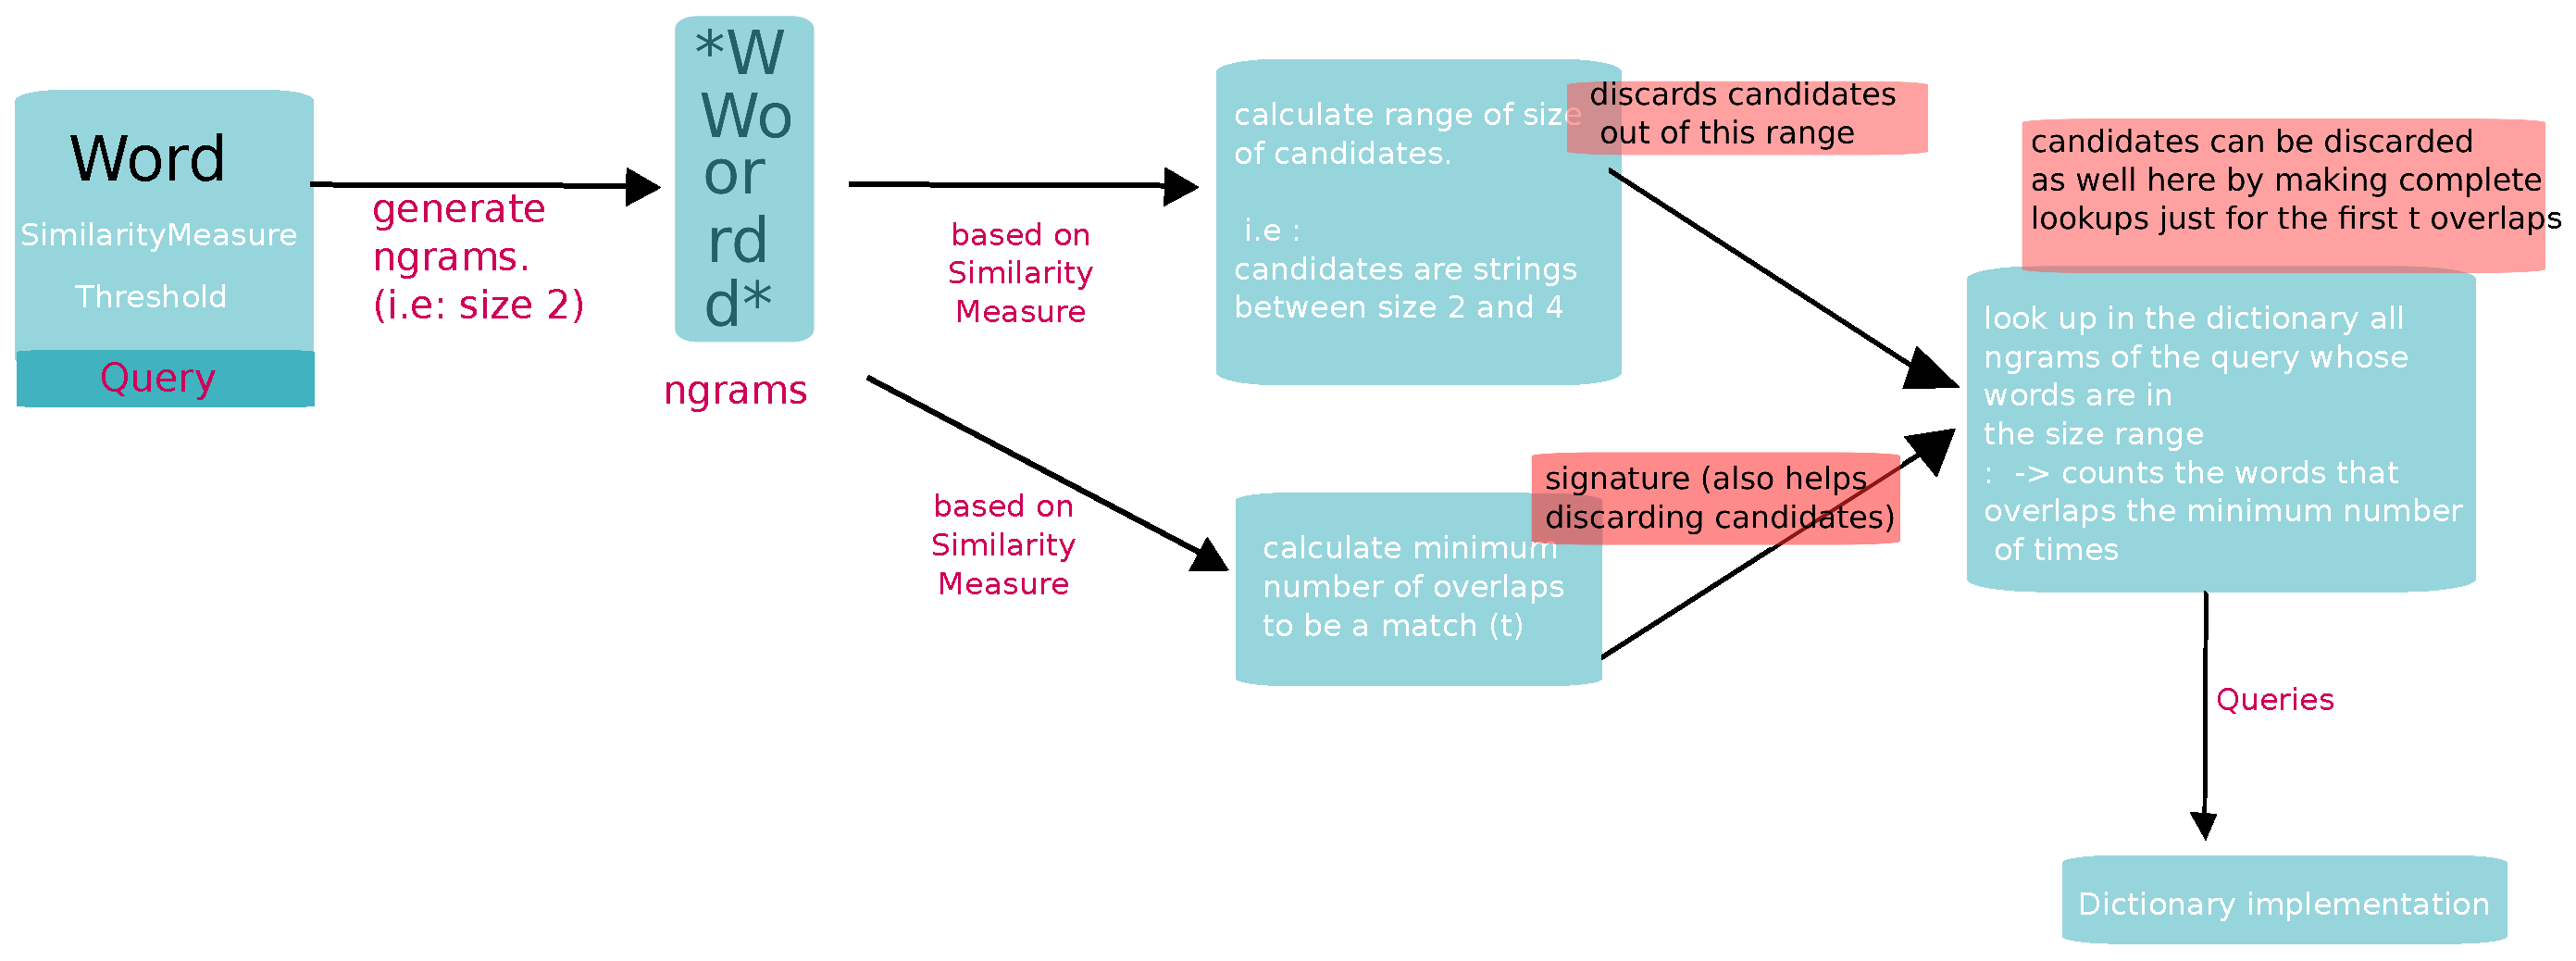
\includegraphics[scale=0.45]{graphics/simStringAlgorithm}
 \caption{Overview of the SimString Algorithm}
  \label{fig:simStringAlgorithm}  
\end{figure}

\end{landscape}


%\newpage

\section{Implementation}
\label{sec:implementation}
The memory mapped hashtable comes with a memory cost, that is since the speed of  a hashtable is to be kept but it will be stored in different files, then a lot of markers and a fix offset of bytes has to be used in order to assure what is in each slot, this means extra memory will be necessary when compared ot the other dictionaries implementations.

To developers NerSimString was implemented in such way so that adding a new dictionary implementation is ndependant of the simString algorithm, in such way new experiments and datastructures can be added.




%\newpage

\section{Evaluation and Results}
\label{sec:results}
\texttt{NERSimString} algorithm with three different dictionary implementations were evaluated by using the CoNLL-2003 Shared Task Data Corpus\footnote{Data files available at: http://www.clips.ua.ac.be/conll2003/ner/} \footnote{English data set request from: http://trec.nist.gov/data/reuters/reuters.html}. We compared the dictionary implementation models against the original SimString algorithm implementation as the baseline. The evaluation of these different implementations measured the average processing time\//\textit{per second} of the dictionaries by considering the given \texttt{n-gram} sizes and different similarity \texttt{thresholds}.

We evaluated these dictionaries on two different CoNLL data settings, only for PER (\textit{person\_NE}) Named Entity type:
\begin{enumerate}[i.]
	\item First, we tested the dictionaries by taking 200 \textbf{random} search strings per method.
	\item Second, we tested the dictionaries by taking the first 200 words from the CoNLL corpus.
\end{enumerate}

The following tables show the results for the average processing times returned by each of the dictionary implementations:

\begin{center}

\begin{table}[H]
\scalebox{0.9}{
  \begin{tabular}{| l | c | c | c | c | r| }
    
    \hline
    \textbf{ } & \textbf{SuffixTree} & \textbf{HashTable} & \textbf{Mapped HashTable} & \textbf{SimString}\\ \hline
    \texttt{Threshold} & 0.2 & 0.2 & 0.2 & 0.2   \\ \hline
    \texttt{N-Gram:3-Avg.Time} & 0.26034846156 & 0.1600577245 & 0.38093002297 & 0.1198204536   \\ \hline
    \texttt{N-Gram:5-Avg.Time} & 0.13545810821 & 0.1907321242 & 0.13516753774 & -   \\ \hline
    \texttt{N-Gram:8-Avg.Time} & 0.18630211667 & 0.1774560892 & 0.19634142339 & -   \\ \hline

    \hline
  \end{tabular}
  }
  \caption{Average Look-up Time Results Based on 200 Random Strings}
  \end{table}
  
\end{center}

\begin{center}

\begin{table}[H]
\scalebox{0.9}{
  \begin{tabular}{| l | c | c | c | c | r| }
    
    \hline
    \textbf{ } & \textbf{SuffixTree} & \textbf{HashTable} & \textbf{Mapped HashTable} & \textbf{SimString}\\ \hline
    \texttt{Threshold} & 0.8 & 0.8 & 0.8 & 0.8   \\ \hline
    \texttt{N-Gram:3-Avg.Time} &   0.317907188  & 0.611821308 & 1.132227919 & 2.774974599   \\ \hline
    \texttt{N-Gram:5-Avg.Time} &   0.448093155  & 0.599589026 & 1.480562861 & -   \\ \hline
    \texttt{N-Gram:8-Avg.Time} &   1.003509663  & 2.200090178 & 1.927359551 & -   \\ \hline
    
    \hline
  \end{tabular}
  }
  \caption{Average Look-up Time Results Based on First 200 Strings on CoNLL Data}
  \end{table}  
\end{center}

These results show that the \texttt{SuffixTree} and the regular\textit{(naive)} \texttt{HashTable} Dictionary implementation outputs were relatively close to the original \texttt{SimString} algorithm implementation. The \texttt{Mapped HashTable} Dictionary handled the data input efficiently as well, however due to the construction of memory mapped structure, the average look-up times resulted in more time than the other two dictionary implementations.



	
	
%\newpage

\section{Conclusion and Future Work}
\label{sec:conclusion}
On this paper, we presented different implementations of the proposed \texttt{SimString} algorithm. We found out that the implementation of \texttt{SimString} is easily extensible for different approaches. Some of the implementations are more useful for other tasks like fast look-up, and for Named Entity Recognition, which is one of the problematic areas in natural language processing and information extraction. We found out that the \texttt{SuffixTree} and \texttt{HashTable} dictionaries returned the relatively similar and fast average look-up times for potential Named Entity candidates. With the different implementations of the inverted dictionary indexes we have presented, we can conclude that they provide different applications, and they were useful in evaluating the performance of the implementation for comparison purposes.\\

Some of the research areas that can be looked further in detail, for example, would be building a \texttt{bootstrapper} for learning Named Entities based on the different implementations of the \texttt{SimString} algorithm, such as the \texttt{NERSimString} dictionaries we presented on this paper. Adding extra similarity measures alternatives for testing and training might also help finding out the best approach for that kind of applications.\\

More sophisticated NER systems can benefit from the \texttt{SimString} implementations by further expanding it with \textit{signature information} which can be extracted from the dictionaries. This info could include anything from finding the \textit{upper and lower boundaries} of NE candidates to applying Noun-Phrase Chunking on the NE Candidates returned from the dictionaries.\\

Besides the potential \textit{bootstrapping} oriented implementation or more sophisticated NER system; adding more support for \texttt{Memory-Mapped HashTable} dictionaries might also be useful for other applications. For the basic NER system, it is expected to see that the \texttt{Mapped HashTable} Dictionaries outputted the slowest search look-up times for Named Entity candidates. However, this does not mean that the \texttt{Mapped HashTable} dictionaries are not a good candidate implementation for other look-up applications, that require a lot of data to be held on the memory. For example, for spell-checker application dictionaries, especially for languages with a large lexicon \textit{(e.g., highly-inflected languages)}, the use of \texttt{Mapped HashTable} dictionary implementation would be very beneficial.\\

Another functionality could be easily added in order to improve this algorithm when searching for Name Entities,
that is for example saving extra information, (a small simstring dictionary for example) with signatures for allowing a better candidate selection with dealing with this task.
When it comes to this task, the simstring structure could also be extended for holding more than one value per key,this  allowing a single dictionary to hold different kinds of name entities.\\

As a final note, for this project, we would like note that researching about different implementation techniques and learning about the differences in application to search look-up was an enjoyable learning task. Because information extracting and search techniques is one of the most challenging--and at the same time rewarding tasks in NLP, we plan on continuing on working on the mentioned research areas for future research.
%\newpage
\bibliographystyle{plain}
\bibliography{simString}
\end{document}